\section{The $RLC$ Circuit}

\noindent
In this section we consider the {\color{blue}\it $RLC$ circuit\/}, shown schematically in
Figure~\ref{figure:6.3.1}. As we'll see, the $RLC$ circuit is an electrical analog of a spring-mass
system with damping.

Nothing happens while the switch is open (dashed line). When the switch is closed (solid line) we
say that the {\color{blue}\it circuit is closed\/}. Differences in electrical potential in a closed
circuit cause current to flow in the circuit. The battery or generator in Figure~\ref{figure:6.3.1}
creates a difference in electrical potential $E=E(t)$ between its two terminals, which we've marked
arbitrarily as positive and negative. (We could just as well interchange the markings.) We'll say
that $E(t)>0$ if the potential at the positive terminal is greater than the potential at the
negative terminal, $E(t)<0$ if the potential at the positive terminal is less than the potential at
the negative terminal, and $E(t)=0$ if the potential is the same at the two terminals. We call $E$
the {\color{blue}\it impressed voltage\/}.

\begin{figure}[H]
  \centering
  \color{blue}
  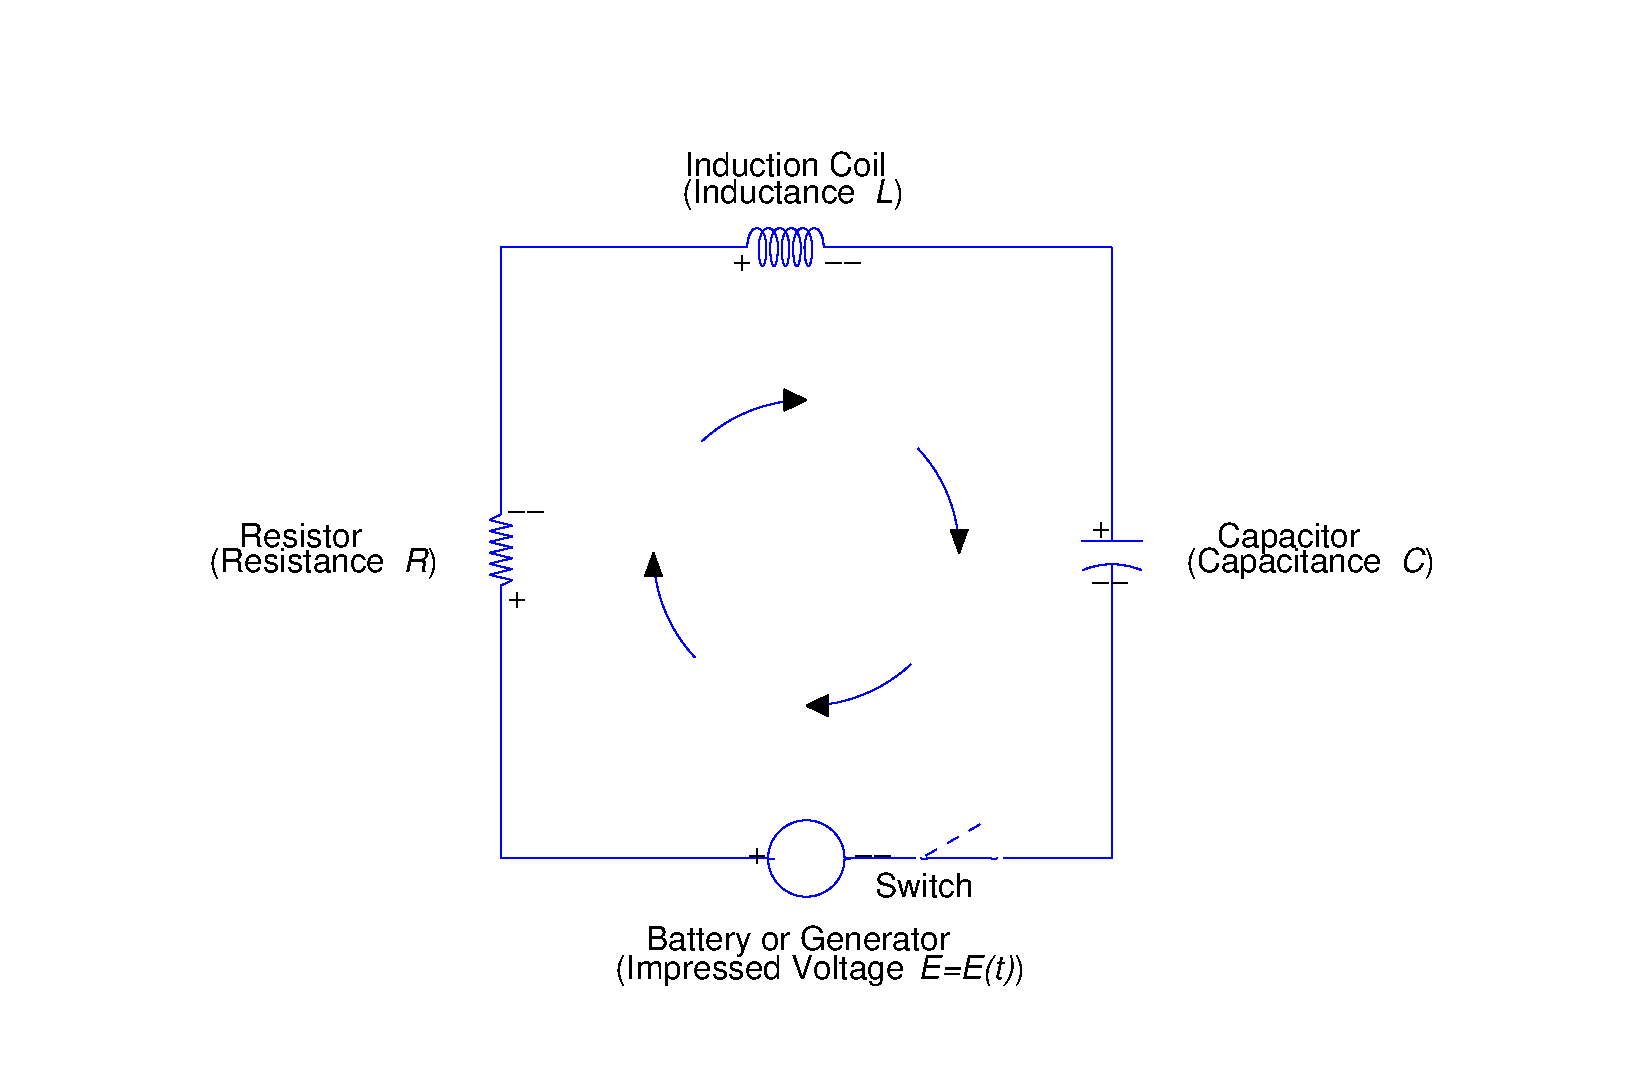
\includegraphics[bb=-78 148 689 643, width=5.67in, height=3.66in, keepaspectratio]{fig060301}
  \caption{An $RLC$ circuit}
  \label{figure:6.3.1}
\end{figure}

At any time $t$, the same current flows in all points of the circuit. We denote current by $I=I(t)$.
We say that $I(t)>0$ if the direction of flow is around the circuit from the positive terminal of
the battery or generator back to the negative terminal, as indicated by the arrows in
Figure~\ref{figure:6.3.1}; $I(t)<0$ if the flow is in the opposite direction, and $I(t)=0$ if no
current flows at time $t$.

Differences in potential occur at the resistor, induction coil, and capacitor in
Figure~\ref{figure:6.3.1}. Note that the two sides of each of these components are also identified
as positive and negative. The {\color{blue}\it voltage drop across\/} each component is defined to
be the potential on the positive side of the component minus the potential on the negative side.
This terminology is somewhat misleading, since ``drop'' suggests a decrease even though changes in
potential are signed quantities and therefore may be increases. Nevertheless, we'll go along with
tradition and call them voltage drops. The voltage drop across the resistor in
Figure~\ref{figure:6.3.1} is given by
\begin{equation}
  \label{eq:6.3.1}V_{R}=IR,
\end{equation}
where $I$ is current and $R$ is a positive constant, the {\color{blue}\it resistance\/} of the
resistor. The voltage drop across the induction coil is given by
\begin{equation}
  \label{eq:6.3.2}V_{I}=L\frac{dI}{dt}=LI',
\end{equation}
where $L$ is a positive constant, the {\color{blue}\it inductance\/} of the coil.

A capacitor stores electrical charge $Q=Q(t)$, which is related to the current in the circuit by the
equation
\begin{equation}
  \label{eq:6.3.3}Q(t)=Q_{0}+\int_{0}^{t}I(\tau)\,d\tau,
\end{equation}
where $Q_{0}$ is the charge on the capacitor at $t=0$. The voltage drop across a capacitor is given
by
\begin{equation}
  \label{eq:6.3.4}V_{C}=\frac{Q}{C},
\end{equation}
where $C$ is a positive constant, the {\color{blue}\it capacitance\/} of the capacitor.

Table~\ref{table:6.3.1} names the units for the quantities that we've discussed. The units are
defined so that
\begin{eqnarray*}
  1\mbox{\,volt}   & = & 1\mbox{\,ampere}\cdot1\mbox{\,ohm}                 \\
                   & = & 1\mbox{\,henry}\cdot1\,\mbox{ampere}/\mbox{second} \\
                   & = & 1\mbox{\,coulomb}/\mbox{\,farad}                   \\[2\jot]
  \arraytext{and}                                                           \\
  1\mbox{\,ampere} & = & 1\mbox{\,coulomb}/\mbox{second}.
\end{eqnarray*}

\medskip
\begin{newtable}
  \label{table:6.3.1} Electrical Units
  \begin{center}
    \begin{tabular}{|c|c|c|}
      \hline
      {\bf Symbol} & {\bf Name}        & {\bf Unit} \\
      \hline
      $E$          & Impressed Voltage & volt       \\
      \hline
      $I$          & Current           & ampere     \\
      \hline
      $Q$          & Charge            & coulomb    \\
      \hline
      $R$          & Resistance        & ohm        \\
      \hline
      $L$          & Inductance        & henry      \\
      \hline
      $C$          & Capacitance       & farad      \\
      \hline
    \end{tabular}
  \end{center}
\end{newtable}

According to \href{https://mathshistory.st-andrews.ac.uk/Biographies/Kirchhoff/}{\color{blue}
\it Kirchhoff's law\/}, the sum of the voltage drops in a closed $RLC$ circuit equals the impressed
voltage. Therefore, from (\ref{eq:6.3.1}), (\ref{eq:6.3.2}), and (\ref{eq:6.3.4}),
\begin{equation}
  \label{eq:6.3.5}LI'+RI+\frac{1}{C}Q=E(t).
\end{equation}
This equation contains two unknowns, the current $I$ in the circuit and the charge $Q$ on the
capacitor. However, (\ref{eq:6.3.3}) implies that $Q'=I$, so (\ref{eq:6.3.5}) can be converted into
the second order equation
\begin{equation}
  \label{eq:6.3.6}LQ''+RQ'+\frac{1}{C}Q=E(t)
\end{equation}
in $Q$. To find the current flowing in an $RLC$ circuit, we solve (\ref{eq:6.3.6}) for $Q$ and then
differentiate the solution to obtain $I$.

In Sections~6.1 and 6.2 we encountered the equation
\begin{equation}
  \label{eq:6.3.7}my''+cy'+ky=F(t)
\end{equation}
in connection with spring-mass systems. Except for notation this equation is the same as
(\ref{eq:6.3.6}). The correspondence between electrical and mechanical quantities connected with
(\ref{eq:6.3.6}) and (\ref{eq:6.3.7}) is shown in Table~\ref{table:6.3.2}.

\blankbox{ \medskip \begin{newtable}\label{table:6.3.2} Electrical and Mechanical Units \begin{center}\begin{tabular}{|lc|lc|}\hline \multicolumn{2}{|c|}{\bf Electrical}& \multicolumn{2}{c|}{\bf Mechanical}\\\hline charge& $Q$& displacement&$y$\\\hline current&$I$&velocity&$y'$\\\hline impressed voltage&$E(t)$&external force&$F(t)$\\\hline inductance&$L$&Mass&$m$\\\hline resistance&$R$&damping&$c$\\\hline 1/capacitance&$1/C$&spring constant&$k$\\\hline\end{tabular}\end{center}\end{newtable}}

\medskip
The equivalence between (\ref{eq:6.3.6}) and (\ref{eq:6.3.7}) is an example of how mathematics
unifies fundamental similarities in diverse physical phenomena. Since we've already studied the
properties of solutions of (\ref{eq:6.3.7}) in Sections~6.1 and 6.2, we can obtain results
concerning solutions of (\ref{eq:6.3.6}) by simply changing notation, according to
Table~\ref{table:6.3.2}.

\boxit{Free Oscillations}

\noindent
We say that an $RLC$ circuit is in {\color{blue}\it free oscillation\/} if $E(t)=0$ for $t>0$, so
that (\ref{eq:6.3.6}) becomes
\begin{equation}
  \label{eq:6.3.8}LQ''+RQ'+\frac{1}{C}Q=0.
\end{equation}
The characteristic equation of (\ref{eq:6.3.8}) is
\[
  Lr^{2}+Rr+\frac{1}{C}=0,
\]
with roots
\begin{equation}
  \label{eq:6.3.9}r_{1}=\frac{-R-\sqrt{R^{2}-4L/C}}{2L}\mbox{\quad and \quad}r_{2}= \frac{-R+\sqrt{R^{2}-4L/C}}{2L}.
\end{equation}
There are three cases to consider, all analogous to the cases considered in Section~6.2 for free
vibrations of a damped spring-mass system.

{\sc Case 1.} The oscillation is {\color{blue}\it underdamped\/} if $R<\sqrt{4L/C}$. In this case,
$r_{1}$ and $r_{2}$ in (\ref{eq:6.3.9}) are complex conjugates, which we write as
\[
  r_{1}=-\frac{R}{2L}+i\omega_{1}\mbox{\quad and \quad}r_{2}=-\frac{R}{2L}-i\omega_{1},
\]
where
\[
  \omega_{1}=\frac{\sqrt{4L/C-R^{2}}}{2L}.
\]
The general solution of (\ref{eq:6.3.8}) is
\[
  Q=e^{-Rt/2L}(c_{1}\cos\omega_{1}t+c_{2}\sin\omega_{1}t),
\]
which we can write as
\begin{equation}
  \label{eq:6.3.10}Q=Ae^{-Rt/2L}\cos(\omega_{1}t-\phi),
\end{equation}
where
\[
  A=\sqrt{c_{1}^{2}+c_{2}^{2}},\quad A\cos\phi=c_{1},\mbox{\quad and \quad}A\sin\phi=c_{2}.
\]
In the idealized case where $R=0$, the solution (\ref{eq:6.3.10}) reduces to
\[
  Q=A\cos\left(\frac{t}{\sqrt{LC}}-\phi\right),
\]
which is analogous to the simple harmonic motion of an undamped spring-mass system in free
vibration.

Actual $RLC$ circuits are usually underdamped, so the case we've just considered is the most
important. However, for completeness we'll consider the other two possibilities.

{\sc Case 2.} The oscillation is {\color{blue}\it overdamped\/} if $R>\sqrt{4L/C}$. In this case,
the zeros $r_{1}$ and $r_{2}$ of the characteristic polynomial are real, with $r_{1}<r_{2}<0$ (see
(\ref{eq:6.3.9})), and the general solution of (\ref{eq:6.3.8}) is
\begin{equation}
  \label{eq:6.3.11}Q=c_{1}e^{r_{1}t}+c_{2}e^{r_{2}t}.
\end{equation}

{\sc Case 3.} The oscillation is {\color{blue}\it critically damped\/} if $R=\sqrt{4L/C}$. In this
case, $r_{1}=r_{2}=-R/2L$ and the general solution of (\ref{eq:6.3.8}) is
\begin{equation}
  \label{eq:6.3.12}Q=e^{-Rt/2L}(c_{1}+c_{2}t).
\end{equation}

If $R>0$, the exponents in (\ref{eq:6.3.10}), (\ref{eq:6.3.11}), and (\ref{eq:6.3.12}) are
negative, so the solution of any homogeneous initial value problem
\[
  LQ''+RQ'+\frac{1}{C}Q=0,\quad Q(0)=Q_{0},\quad Q'(0)=I_{0},
\]
approaches zero exponentially as $t\to\infty$. Thus, all such solutions are {\color{blue}\it
transient\/}, in the sense defined Section~6.2 in the discussion of forced vibrations of a
spring-mass system with damping.

\begin{example}
  \label{example:6.3.1} \rm At $t=0$ a current of 2 amperes flows in an $RLC$ circuit with
  resistance $R=40$ ohms, inductance $L=.2$ henrys, and capacitance $C=10^{-5}$ farads. Find the
  current flowing in the circuit at $t>0$ if the initial charge on the capacitor is 1 coulomb.
  Assume that $E(t)=0$ for $t>0$.
\end{example}

\solution The equation for the charge $Q$ is
\[
  \frac{1}{5}Q''+40Q'+10000Q=0,
\]
or
\begin{equation}
  \label{eq:6.3.13}Q''+200Q'+50000Q=0.
\end{equation}
Therefore we must solve the initial value problem
\begin{equation}
  \label{eq:6.3.14}Q''+200Q'+50000Q=0,\quad Q(0)=1,\quad Q'(0)=2.
\end{equation}
The desired current is the derivative of the solution of this initial value problem.

The characteristic equation of (\ref{eq:6.3.13}) is
\[
  r^{2}+200r+50000=0,
\]
which has complex zeros $r=-100\pm200i$. Therefore the general solution of (\ref{eq:6.3.13}) is
\begin{equation}
  \label{eq:6.3.15}Q=e^{-100t}(c_{1}\cos200t+c_{2}\sin200t).
\end{equation}
Differentiating this and collecting like terms yields
\begin{equation}
  \label{eq:6.3.16}Q'=-e^{-100t}\left[(100c_{1}-200c_{2})\cos200t+ (100c_{2}+200c_{1})\sin200t\right].
\end{equation}
To find the solution of the initial value problem (\ref{eq:6.3.14}), we set $t=0$ in
(\ref{eq:6.3.15}) and (\ref{eq:6.3.16}) to obtain
\[
  c_{1}=Q(0)=1\mbox{\quad and \quad}-100c_{1}+200c_{2}=Q'(0)=2;
\]
therefore, $c_{1}=1$ and $c_{2}=51/100$, so
\[
  Q=e^{-100t}\left(\cos200t+\frac{51}{100}\sin200t\right)
\]
is the solution of (\ref{eq:6.3.14}). Differentiating this yields
\[
  I=e^{-100t}(2\cos200t-251\sin200t).
\]

\boxit{Forced Oscillations With Damping}

\noindent
An initial value problem for (\ref{eq:6.3.6}) has the form
\begin{equation}
  \label{eq:6.3.17}LQ''+RQ'+\frac{1}{C}Q=E(t),\quad Q(0)=Q_{0},\quad Q'(0)=I_{0},
\end{equation}
where $Q_{0}$ is the initial charge on the capacitor and $I_{0}$ is the initial current in the
circuit. We've already seen that if $E\equiv0$ then all solutions of (\ref{eq:6.3.17}) are
transient. If $E\not\equiv0$, we know that the solution of (\ref{eq:6.3.17}) has the form
$Q=Q_{c}+Q_{p}$, where $Q_{c}$ satisfies the complementary equation, and approaches zero
exponentially as $t\to\infty$ for any initial conditions , while $Q_{p}$ depends only on $E$ and is
independent of the initial conditions. As in the case of forced oscillations of a spring-mass system
with damping, we call $Q_{p}$ the {\color{blue}\it steady state\/} charge on the capacitor of the
$RLC$ circuit. Since $I=Q'=Q_{c}'+Q_{p}'$ and $Q_{c}'$ also tends to zero exponentially as
$t\to\infty$, we say that $I_{c}=Q'_{c}$ is the {\color{blue}\it transient\/} current and
$I_{p}=Q_{p}'$ is the {\color{blue}\it steady state\/} current. In most applications we're
interested only in the steady state charge and current.

\begin{example}
  \label{example:6.3.2} \rm Find the amplitude-phase form of the steady state current in the $RLC$
  circuit in Figure~\ref{figure:6.3.1} if the impressed voltage, provided by an alternating current
  generator, is $E(t)=E_{0}\cos\omega t$.
\end{example}

\solution We'll first find the steady state charge on the capacitor as a particular solution of
\[
  LQ''+RQ'+\frac{1}{C}Q=E_{0}\cos\omega t.
\]
To do this, we'll simply reinterpret a result obtained in Section~6.2, where we found that the
steady state solution of
\[
  my''+cy'+ky=F_{0}\cos\omega t
\]
is
\[
  y_{p}=\frac{F_{0}}{\sqrt{(k-m\omega^{2})^{2}+c^{2}\omega^{2}}}\cos(\omega t-\phi),
\]
where
\[
  \cos\phi=\frac{k-m\omega^{2}}{\sqrt{(k-m\omega^{2})^{2}+c^{2}\omega^{2}}}\mbox{\quad and \quad}\sin\phi=\frac{c\omega}{\sqrt{(k-m\omega^{2})^{2}+c^{2}\omega^{2}}}.
\]
(See Equations~\eqref{eq:6.2.14} and \eqref{eq:6.2.15}.) By making the appropriate changes in the
symbols (according to Table~\ref{table:6.3.2}) we obtain the steady state charge
\[
  Q_{p}=\frac{E_{0}}{\sqrt{(1/C-L\omega^{2})^{2}+R^{2}\omega^{2}}}\cos(\omega t-\phi),
\]
where
\[
  \cos\phi=\frac{1/C-L\omega^{2}}{\sqrt{(1/C-L\omega^{2})^{2}+R^{2}\omega^{2}}}\mbox{\quad and \quad}\sin\phi=\frac{R\omega}{\sqrt{(1/C-L\omega^{2})^{2}+R^{2}\omega^{2}}}.
\]
Therefore the steady state current in the circuit is
\[
  I_{p}=Q_{p}'= -\frac{\omega E_{0}}{\sqrt{(1/C-L\omega^{2})^{2}+R^{2}\omega^{2}}}\sin(\omega t-\phi).
\]

\exercises In Exercises~\ref{exer:6.3.1}-\ref{exer:6.3.5} find the current in the $RLC$ circuit, assuming that $E(t)=0$ for $t>0$.

\begin{exerciselist}
  \item\label{exer:6.3.1} $R=3$ ohms; \, $L=.1$ henrys; \, $C=.01$ farads; $Q_{0}=0$ coulombs;
        \,$I_{0}=2$ amperes.

  \item\label{exer:6.3.2} $R=2$ ohms; \, $L=.05$ henrys; \, $C=.01$ farads; $Q_{0}=2$ coulombs;
        \,$I_{0}=-2$ amperes.

  \item\label{exer:6.3.3} $R=2$ ohms; \, $L=.1$ henrys; \, $C=.01$ farads; $Q_{0}=2$ coulombs;
        \,$I_{0}=0$ amperes.

  \item\label{exer:6.3.4} $R=6$ ohms; \, $L=.1$ henrys; \, $C=.004$ farads; $Q_{0}=3$ coulombs;
        \,$I_{0}=-10$ amperes.

  \item\label{exer:6.3.5} $R=4$ ohms; \, $L=.05$ henrys; \, $C=.008$ farads; $Q_{0}=-1$ coulombs;
        \,$I_{0}=2$ amperes.

  \exercisetext{In Exercises~\ref{exer:6.3.6}-\ref{exer:6.3.10} find the steady state current in the
  circuit described by the equation.}

  \item\label{exer:6.3.6} $\dst\frac{1}{10}Q''+3Q'+100Q=5\cos10t-5\sin10t$

  \item\label{exer:6.3.7} $\dst\frac{1}{20}Q''+2Q'+100Q=10\cos25t-5\sin25t$

  \item\label{exer:6.3.8} $\dst\frac{1}{10}Q''+2Q'+100Q=3\cos50t-6\sin50t$

  \item\label{exer:6.3.9} $\dst\frac{1}{10}Q''+6Q'+250Q=10\cos100t+30\sin100t$

  \item\label{exer:6.3.10} $\dst\frac{1}{20}Q''+4Q'+125Q=15\cos30t-30\sin30t$

  \item\label{exer:6.3.11} Show that if $E(t)=U\cos\omega t+V\sin\omega t$ where $U$ and $V$ are
        constants then the steady state current in the $RLC$ circuit shown in
        Figure~\ref{figure:6.3.1} is
  \[
    I_{p}=\frac{\omega^{2}RE(t)+(1/C-L\omega^{2})E'(t)}{\Delta},
  \]
  where
  \[
    \Delta=(1/C-L\omega^{2})^{2}+R^{2}\omega^{2}.
  \]

  \item\label{exer:6.3.12} Find the amplitude of the steady state current $I_{p}$ in the $RLC$
        circuit shown in Figure~\ref{figure:6.3.1} if $E(t)=U\cos\omega t+V\sin\omega t$, where $U$
        and $V$ are constants. Then find the value $\omega_{0}$ of $\omega$ that maximizes the amplitude,
        and find the maximum amplitude.

  \exercisetext{In Exercises~\ref{exer:6.3.13}-\ref{exer:6.3.17} plot the amplitude of the steady
  state current against $\omega$. Estimate the value of $\omega$ that maximizes the amplitude of the
  steady state current, and estimate this maximum amplitude. \hint{You can confirm your results by
  doing Exercise~\ref{exer:6.3.12}.}}

  \item\label{exer:6.3.13} \Lex $\dst\frac{1}{10}Q''+3Q'+100Q=U\cos\omega t+V\sin\omega t$

  \item\label{exer:6.3.14} \Lex $\dst\frac{1}{20}Q''+2Q'+100Q=U\cos\omega t+V\sin\omega t$

  \item\label{exer:6.3.15} \Lex $\dst\frac{1}{10}Q''+2Q'+100Q=U\cos\omega t+V\sin\omega t$

  \item\label{exer:6.3.16} \Lex $\dst\frac{1}{10}Q''+6Q'+250Q=U\cos\omega t+V\sin\omega t$

  \item\label{exer:6.3.17} \Lex $\dst\frac{1}{20}Q''+4Q'+125Q=U\cos\omega t+V\sin\omega t$
\end{exerciselist}
